\documentclass[3p,twocolumn]{elsarticle}

\usepackage{graphicx}
\usepackage{color}
\usepackage{amsmath}
\usepackage{amssymb}
\usepackage{amsfonts}
\usepackage{float}
\usepackage{supertabular}
%\usepackage{multicol}
\usepackage{hyperref}
\usepackage{float}

% give the macro \cref
\usepackage{cleveref}

%allow custom hyphenation
\usepackage{hyphenat}

%\floatstyle{simplerule}
%\newfloat{floatbox}{thp}{lob}[section]
%\floatname{floatbox}{Text Box}

% corrections
%\newcommand{\E}[1]{\textcolor{red}{\textbf{{#1}}}}
%\newcommand{\C}[1]{\textcolor{blue}{\textbf{{#1}}}}
%\newenvironment{ERIK}{\color{red}}{\color{black}}
%\newenvironment{CARLI}{\color{blue}}{\color{black}}


\begin{document}

\title{HASEonGPU}

\author[hzdr]{C. Eckert}
\ead{c.eckert@hzdr.de}

\author[hzdr]{E. Zenker}
\ead{e.zenker@hzdr.de}

\author[hzdr]{D. Albach}
\ead{d.albach@hzdr.de}

\author[hzdr]{M. Bussmann}
\ead{m.bussmann@hzdr.de}

\address[hzdr]{
  Institute of Radiation Physics, 
  Helmholtz-Zentrum Dresden-Rossendorf e. V.,
  Bautzner Landstra\ss e 400,
  01328 Dresden,  
  Germany
}


%abstract must be before maketitle
\hyphenation{MATLAB}
\hyphenation{NVIDIA}
\hyphenation{README}

\begin{abstract}
  A fast GPU-implementation of a MonteCarlo based ASE-Flux simulation.
\end{abstract}


\maketitle

%\begin{multicols}{2}

\section{Introduction}
\numberwithin{equation}{section}

Any excited upper laser state will inevitably emit spontaneously photons due
its radiative life time. Those photons freely travel within the gain medium
itself and experience amplification. This process can drastically reduce the
stored energy and is called Amplified Spontaneous Emission (ASE). ASE does not
only reduce locally stored energy, it dislocates energy into not pumped areas,
like sourrounding claddings or mounts. Therefore it has to be considered as an
important factor for heat distribution inside and outside of the pumped laser
gain medium.

Together with laser induced damage and thermal related issues is ASE one of the
challenges for every laser gain medium design to overcome. The impact of ASE on
energy storage has been studied since the early days of lasers [1,2,3].
However, with the increasing importance of diode pumped lasers, this particular
topic came in the focus of interest again [4,5].

For most of the applied cases ASE and related problems cannot be treated
analytically and is therefore subject to numerical analysis. Most numerical
codes usually simplify the problem in order to gain computation time. With the
advent of GPU based codes, it is of strong interest to take advantage of the
good scalability of the Monte-Carlo approach used in our recent model [4].

In this paper we concentrate on the adaptation, extention and performance
increase of the model described and benchmarked in [4].

\section{Model}

This section describes the underlying model and ideas for the $\Phi_{ASE}$
calculation in an active gain medium with planar top and bottom surfaces (see
figure \ref{graphic:samples_reduced}).



\subsection{The crystal mesh} \label{subsec:meshSampling}

To distribute the \emph{sample points} on the medium, it is seen as a
horizontal 2-dimensional plane, which can be sampled with a non-uniform
density. This approach allows to increase the spatial resolution in certain
areas of interest. Using Delauny triangulation, these sample points are
connected to a 2D mesh of triangles.

The triangle mesh is extruded in direction of the vertical axis to form a
\emph{slice} of right prisms (figure \ref{graphic:extruded_mesh}). This
slice is then duplicated several times, until the whole medium is divided into
prisms (figure \ref{graphic:samples_reduced}).

\begin{figure}
  \centerline{
    \resizebox{0.5\textwidth} {!} {\includegraphics{graphics/delauny_3.png}}
  }
  \caption{extruded plane of triangles}
  \label{graphic:extruded_mesh}
\end{figure}

\begin{figure}
  \centerline{
    \resizebox{0.5\textwidth} {!} {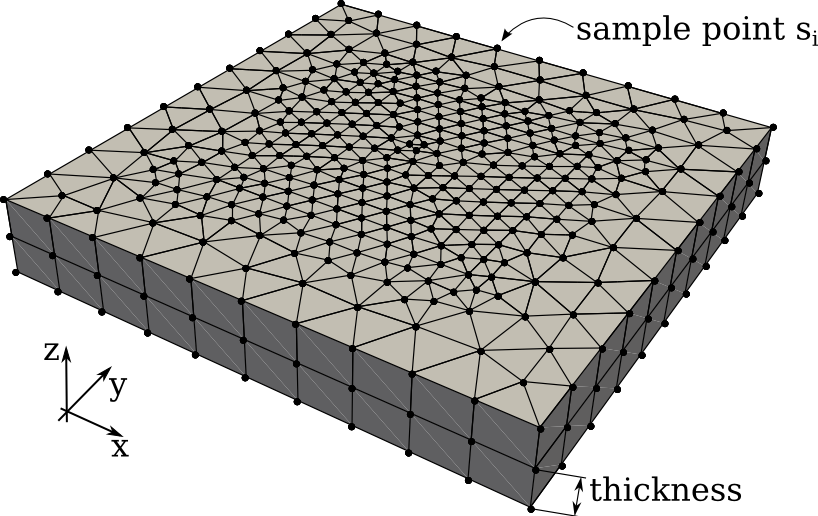
\includegraphics{graphics/samples_reduced.png}}
  }
  \caption{non-uniform sampling of active gain medium in 2 slices}
  \label{graphic:samples_reduced}
\end{figure}




\subsection{Ray tracing}
\label{subsec:raytracing}

To calculate the amplification of a single ray from a position $r_i$ to a sample
point $r_0$, the ray is traced along its path through the prisms (see figure
\ref{graphic:prism_propagation}). 

\begin{figure}[H]
  \centerline{
    \resizebox{0.5\textwidth} {!} {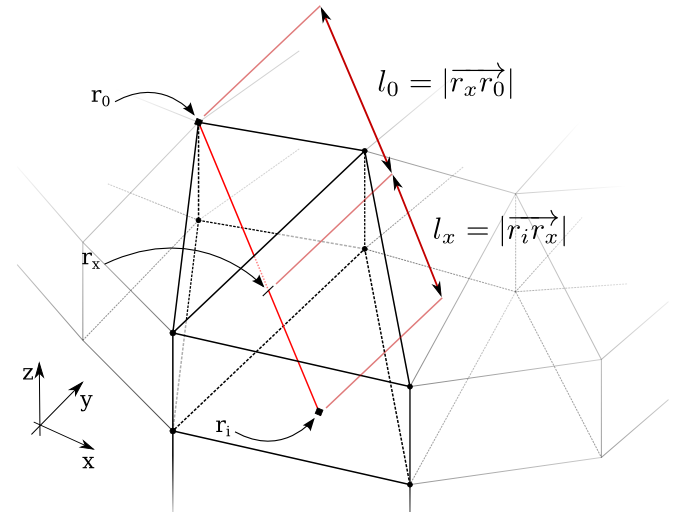
\includegraphics{./graphics/prism_propagation_2.png}}
  }
  \caption{propagation of a ray through the prism structure}
  \label{graphic:prism_propagation}
\end{figure}

Starting from point $r_i$ inside a prism, there are 5 possible intersection
planes for the ray. One plane for the top and bottom surfaces and one for each
of the 3 horizontal sides. Once the intersection plane is determined (the ray is
intersecting at point $r_x$), the next prism can be calculated based on the
knowledge about the meshing structure:

\begin{description}

  \item[horizontal side]
    the ray will remain in the same slice, but the next prism is based on a
    different triangle. This triangle is a \emph{neighbor} of the previous one.
    The relevant datastructure to determine the neighboring triangle is created
    during the Delauny triangulation in \ref{subsec:meshSampling}.

  \item[top/bottom plane]
    if the ray is intersecting with the top or bottom plane of the prism, the
    next prism will be based on the same triangle as before, but in a different
    slice.

\end{description}

This process is iterated for each prism on the path between $r_i$ and the
desired sample point $r_0$. The intersections (like $r_x$) with prism surfaces
define line segments of a certain length $l_x$. These segments are used for the
gain calculation: For each prism $x$, the contribution to the gain is calculated
as a function of $l_x$:

\begin{equation}
\label{eq:partial_gain}
  partial\_gain(x) = 
  e^{N_{tot} \cdot (\beta_x \cdot (\sigma_e + \sigma_a) - \sigma_a)) \cdot l_x}
\end{equation}
where $\beta_x$ is the \textbf{TODO: describe beta} beta value in the current
prism.

The gain for the whole ray can then be computed as

\begin{equation}
\label{eq:gain}
  gain(\overrightarrow{r_ir_0}) =  
  \frac{\beta_i}{ |\overrightarrow{r_ir_0}|^2} \cdot \prod^npartial\_gain(n) 
\end{equation}


\subsection{Reflections}
\label{subsec:reflections}

In order to allow for reflecting rays on the upper and lower surface of the
medium, the model is extended to include the refractive indices of the medium
and the surrounding.  Furthermore, each triangle on the surfaces may be covered
with a different coating material. The ray is split into multiple separate
sub-rays, each representing one part of the reflection (see figure
\ref{graphic:reflections_2D}: $\overrightarrow{r_im_1}$,
$\overrightarrow{m_1m_2}$, $\overrightarrow{m_2r_0}$).


\begin{figure}[H]
  \centerline{
    \resizebox{0.5\textwidth} {!} {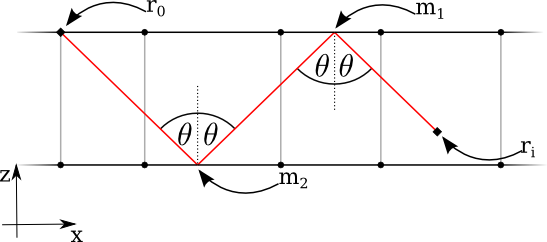
\includegraphics{./graphics/reflections_1.png}}
  }
  \caption{reflections of a ray propagation on the crystal surface}
  \label{graphic:reflections_2D}
\end{figure}


On each of the reflection points, the refractive indices of crystal and
environment are used to determine the maximum angle for a total reflection. This
can now be used to estimate the \emph{initial gain} $g_i$ of a ray that is
reflected at position $x_i$:

\begin{equation}
\label{eq:gain}
  g_i = 
  \begin{cases}
    gain(\overrightarrow{x_{i-1}x_i}) & if \alpha \ge \alpha_{tot}  \\
    gain(\overrightarrow{x_{i-1}x_i}) \cdot \gamma(x_i) & if \alpha < \alpha_{tot}   
  \end{cases}
\end{equation}

This computation comprises a significant overhead, which necessitates the use of
a high performance algorithm. 

However, the current implementation only supports reflections on the upper and
lower surface, resulting in a limitation which excludes the simulation of
lateral lasing.


\subsection{Monte Carlo simulation}
\label{subsec:monteCarlo}

\begin{itemize}

  \item \textit{integral is expressed by formula} \cite[Daniel's Thesis]{ASE2010}

  \item Monte Carlo simulation as a way to calculate the integral for the whole
    crystal.

  \item \textit{formula for the additive Monte Carlo}

\end{itemize}







\section{Methods}
\subsection{Parallel methods}
There are several granularities and ways of parallelization in this kind of 
Monte Carlo simulation. In the following, the used parallelization points and
its implementations are listed:

\begin{description}

  \item[Sample points] (multiple GPUs)\\
    The sample points introduced in \ref{subsec:meshSampling} are independent from each other
    and therefore its $\Phi$-ASE can be calculated in parallel. Every $\Phi$-ASE
    calculation runs in his own GPU-Kernel, thus sample points can be partioned 
    to several devices. As a result the speedup for multiple GPUs is almost linear.

  \item[Rays] (GPU threads)\\
    Every ray can be traced independently through the mesh structure.
    Exploiting this parallelism provides a great opportunity to boost
    performance. Only the resulting gains for each sample point have to be
    added atomatically in the end.
    Furthermore rays with same origin and direction will be grouped
    into warps to utilize the GPU cache in a good way.

  \item[Wavelengths] (Seperate block dimension)\\
    According to \ref{subsec:monteCarlo}, the simulation of a polychromatic
    laser can be split into sufficiently small monochromatic simulations which
    are again completely independent from each other.

\end{description}

\subsection{Importance sampling}
Importance sampling is a well known technique in the domain
of statistics \cite{importanceSamplingSource}. In case of 
ASE-Flux calculation a presampling of a sample point is done
to figure out which areas inside the mesh are worth to start rays from.
This method has a strong impact on the precision of the
simulation.

Figure \ref{graphic:importance} demonstrates
the differences between calculation with und without
importance sampling. It is shown each a cut through the activ 
gain medium in which the graphic without important
sampling has some peaks. Thus importance 
sampling can increase the efficiency of Monte-Carlo-Simulations 
by reducing variance and simulation runtime. 
\begin{figure}
  \centerline
  {\resizebox{0.45\textwidth}{!}{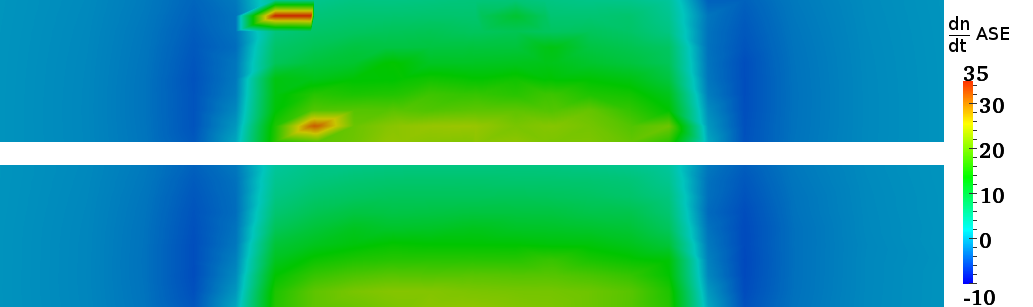
\includegraphics{graphics/importance.png}}}
  \caption{Cuts through activ gain medium: no importance sampling (top), with importance sampling (bottom)}
  \label{graphic:importance}
\end{figure}

\subsection{Adaptive sampling}
Since most sample points behave in a good way, there is no need
to sample them with a high number of rays. Only some outliers need to
be simulated with a higher precision. You can quantify the precision
and therefore the difference between the true and calculated value by
further determine the mean squared error (MSE).
The adaptive method allows you to remove strong peaks in the result
of the simulation without sampling all sample points with
a high number of rays and therefore reduce runtime.
\begin{figure}
  \centerline{
    \resizebox{0.45\textwidth}{!}{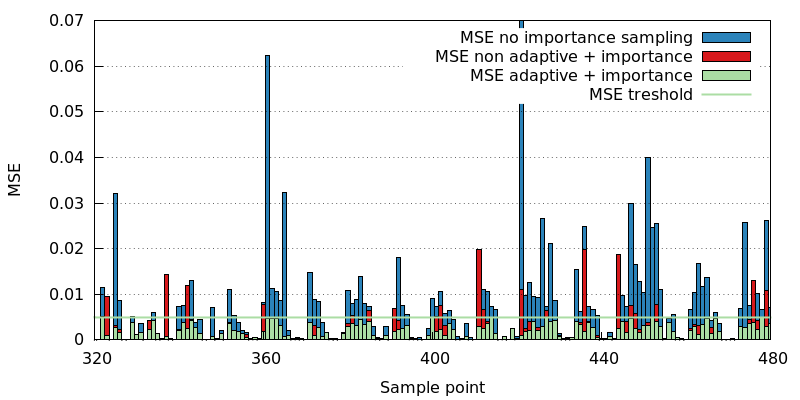
\includegraphics{plot/mse.png}}}
  \caption{Comparision no importance samling, not adaptive, adaptive}
  \label{plot:adaptive}
\end{figure}

In Figure~\ref{plot:adaptive} the adaptive method with 
50K to 500M rays per sample point is compared to the simulations
not adaptive and no importance sampling with each 300K rays per sample point (same runtime of 10s).
The not adaptive and no importance sampling method have some big peaks while all sample points of 
the adaptive method lie under a preset $MSE$-threshold (in this case 0.005). 

The adaptive method won't reduce the average MSE over sample points,
but it will reduce the maximal MSE values. Thus using the adaptives
methods gives higher precision by same calculation time.

%\begin{itemize}
%\item []
%     \[f(\vec{r_0}) = \frac{1}{n} \sum_{i=1}^n g_i \]
%     \[f^2(r_0) = \frac{1}{n} \sum_{i=1}^n g_i^2 \]
%     \[MSE(r_0) = \sqrt{\frac{f^2(r_0) - f(r_0)^2}{n}}\]
%\end{itemize}


\section{Application}
\numberwithin{equation}{section}

The application is available as a commandline-tool and reads
its simulation data from plain text files (in future also from stdin).
For an easy access the offered MATLAB interface (see \ref{label:matlab_interface}) 
is highly recommended. Experienced users can also call the application
directly. Please consult the README file, the provided 
example code or the source code for more details.\\
\textbf{TODO:}~octave interface ?

\subsection{Installation}
The application was tested and developed under a linux environment.
It can be built by running make inside the application directory, provided
that make (up to 3.81), gcc (up to 4.6.2) and cuda (5.0) are installed. 
This will also setup a MATLAB file calcPhiASE.m in the application
directory. The device code runs on Nvida graphics cards from compute 
capability 2.0 (at least fermi generation). 

\subsection{MATLAB interface}
\label{label:matlab_interface}
Because MATLAB is widely used in academic and research institutions, a MATLAB
interface is provided. You need to include the MATLAB file calcPhisASE.m from
the application directory into your MATLAB path and call the calcPhiASE function 
from you MATLAB environment.

\subsubsection{Usage}
In \ref{label:input} you'll find a brief overview about the
arguments of the calcPhisAse function. See the README file for 
more interface details. Otherwise it's just a function call from
your MATLAB script.
\[[phiASE,~MSE,~nRays] = calcPhiASE(args)\]
Mesh information need to be generated in advanced
to save calculation time, because usually $\Phi$-ASE calculations
run over several timesteps on the same mesh. 


%%\subsection{Features}
%%\begin{itemize}
%%  \item polychromatic (multiple wavelengths)
%%  \item reflections on top and bottom of amplifying medium
%%  \item variable + adaptive number of rays per sample point
%%  \item multigpu on one computation node
%%  \item threshold for MSE
%%  \item creation of VTK files containing $\Phi_{ASE}$, reflections per prism etc.
%%  \item comparison with existing VTK files 
%% \end{itemize}



\subsubsection{Input Arguments}
\label{label:input}
\tablehead{\hline \textbf{Argument} & \textbf{Description} \\\hline \hline}
\begin{supertabular}{| p{3cm} | p{4cm} |}
  points & Sample points of the mesh \\\hline
  triangleNormalsX & X coordinates of triangle edges normal vector \\\hline
  triangleNormalsY & Y coordinates of triangle edges normal vector \\\hline
  forbiddenEdges & Adjacent edges of neighbor triangles\\\hline
  triangleNormalPoint & Start points of triangle edges normal vector \\\hline
  triangleNeighbors & Neighbor relation of triangles \\\hline
  trianglePoints & Points of the triangle vertices \\\hline
  thickness & Thickness of one mesh level \\\hline
  numberOfLevels & Total number of levels \\\hline
  nTot & \textbf{TODO} Some constant \\\hline
  betaVol & \textbf{TODO} Some constant for each sample Points \\\hline
  laserWavelength & \textbf{TODO} Laserparameter \\\hline
  crystal & \textbf{TODO}Crystalparameter \\\hline
  prismBetaValues & \textbf{TODO} Some constant for every prism of the mesh \\\hline
  triangleSurfaces & Surfaces of triangles \\\hline
  triangleCenterX & X coordinate of triangle center point\\\hline
  triangleCenterY & Y coordinate of triangle center point\\\hline
  clad & \textbf{TODO} Cladding stuff \\\hline
  cladNum & \textbf{TODO} More Cladding stuff \\\hline
  cladAbs & \textbf{TODO} More Cladding stuff \\\hline
  refractiveIndices &  Refraction index of mesh and volume around \\\hline
  reflectivities & Reflectivities of mesh planes top and bottom \\\hline
  maxRays & Maximal number of rays for adaptive sampling \\\hline
  MSEThreshold & MSE-Threshold for adaptive sampling \\\hline
  useReflections & Switch to activate reflections \\\hline
\end{supertabular}

\subsubsection{Output}
\tablehead{\hline \textbf{Output} & \textbf{Description} \\\hline \hline}
\begin{supertabular}{| p{3cm} | p{4cm} |}
  \hline
  phiASE & solution of simulation for each sample point \\\hline
  MSE & Mean squared error for each sample point \\\hline
  nRays & number of rays per sample point \\\hline
\end{supertabular}

\section{Results}
\numberwithin{equation}{section}

\subsection{Setup of the testing environment}
\label{subsec:testingEnvironment}

The benchmarks were conducted on a GPU cluster consisting of 12 compute nodes,
each equipped with a quad core Intel Xeon CPU E5-2609 CPU (2.40GHz), 64GB RAM
and 4 NVIDIA Tesla K20M GPUs. Each GPU contains 2496 CUDA cores with a total
peak performance of 3520 GFLOP/s. Job submission is handled by TORQUE
(\cite{torque}) with Maui as scheduling backend. The modeled gain medium is a
\textbf{TODO: Daniel should check/complete the description of the medium} YAG
crystal with a square surface of $16cm^2$\textbf{(?)} and a thickness of
$0.6cm$\textbf{(?)}. Its upper surface was sampled with 321 points, resulting in
600 Delaunay triangles (see section \ref{subsec:meshSampling}). The mesh is
extruded 9 times on the vertical axis, amounting to a total of 3210 sample
points and 5400 prisms respectively.

\subsection{Benchmark of values}

\begin{itemize}

  \item TODO

  \item \textbf{Image: gain VS time for one single point. Overlay between
    experiment/daniels sim/our sim}

  \item comparison with previous values from Daniel's thesis

  \item (comparison with results from an experiment)

\end{itemize}


\subsection{Runtimes}
In Figure \ref{plot:runtime}, the runtimes of the original single threaded
algorithm from \cite{ASE2010} are compared to the developed non-adaptive
parallel ASE-flux algorithm with different numbers of rays to demonstrate
scaling for different workloads. All simulations were done without using
reflections. To increase the number of GPUs, MPI\cite{MPI} was used to distribute the
sample points to all available devices. 

%reflections. To increase the number of GPUs to 48, an \emph{array job} was
%scheduled and the sampling points distributed evenly to the 12 Nodes (each
%hosting 4 GPUs) as seen in section \ref{subsubsec:multigpu}. When using the CPU
%or up to 4 GPUs, the computation uses only a single node, which results in a
%linear scaling of the algorithm. If the cluster's job submission system is used,
%a significant runtime overhead can be seen as a result of the job scheduler
%taking several seconds to process a single job. Therefore, using a high number
%of GPUs can lead to suboptimal performance in otherwise fast computations.
%However, this becomes neglegible for very work intensive simulations.
\begin{figure}[H]
  \centerline{
    \resizebox{0.5\textwidth}{!}{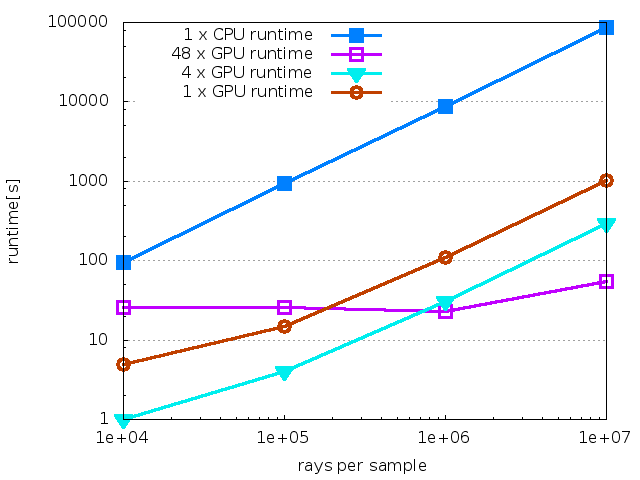
\includegraphics{plot/runtime.png}}}
  \caption{runtime of orginial algorithm compared to parallel algorithm}
  \label{plot:runtime}
\end{figure}
For the adaptive algorithm, simulation times of different sample points can vary
significantly (see Section \ref{subsec:adaptive_sampling}). Therefore, a uniform
partitioning of the sample points among the nodes would result in an unbalanced
workload and reduced efficency for the whole computation. Instead, one of the
nodes acts as a \emph{head node} and manages workload distribution based on demand: As
soon as one of the \emph{compute nodes} is idle, it will request more data to simulate.
Apart from a constant initialization overhead, distributing the computation to
multiple devices scales well, even with the adaptive algorithm. (Figure
\ref{plot:gpu_scaling}).
\begin{figure}[H]
  \centerline{
    \resizebox{0.5\textwidth}{!}{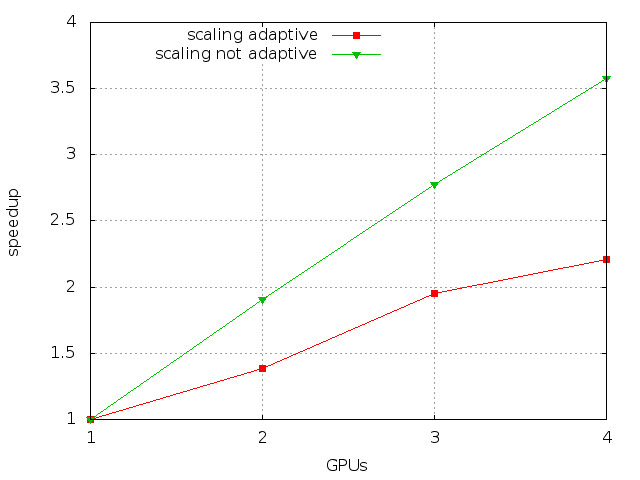
\includegraphics{plot/scaling.png}}}
  \caption{efficiency on multiple devices}
  \label{plot:gpu_scaling}
\end{figure}
Adaptive sampling usually does not only eliminate outliers, but even reduce the
needed time to do so: By using the idea of a pre-defined $MSE$-threshold, the
precision of the simulation can be adjusted in terms of this threshold rather than
simply increasing the number of rays for all the sample points. Since only a
small subset of sample points actually needs to be sampled with a high
resolution, a small increase in runtime can be sufficient to lower the maximal
$MSE$ values below the desired threshold (Figure \ref{plot:adaptive_runtime}).
This can be adjusted to yield similar simulation results as the non-adaptive
implementation at a fraction of its runtime. Note that some values in the
graphic actually display almost the same runtime, since the computation always
succeeded to stay below the given threshold with very little additional effort.
\begin{figure}[H]
  \centerline{
    \resizebox{0.5\textwidth}{!}{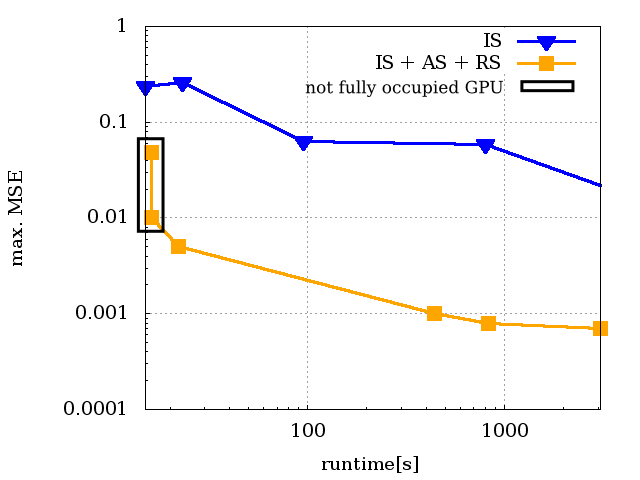
\includegraphics{graphics/adaptive_runtime.png}}}
  \caption{runtime comparison of adaptive and non-adaptive }
  \label{plot:adaptive_runtime}
\end{figure}
\subsection{Limitations and future work}
\label{subsec:limitations}
Future work should address reflections on the lateral sides of the gain medium
to allow the simulation of lateral feedback. The current implementation only
supports reflections on the upper and lower surface. Furthermore, these upper
and lower surfaces need to be coplanar due to the structure of the mesh
(Section \ref{subsec:meshSampling}).
Another limitation originates from the fact that each simulation uses a mapping
from rays to their respective starting position. For a large number of rays,
this can lead to a substancial amout of allocated memory. With the current
hardware (Section \ref{testingEnvironment}) and implementation, each sample
point can be simulated with a maximum of $6.5e8$ rays. To push this limit
further, a more sophisticated mapping needs to be implemented. This could
be done by simply splitting the mapping in different parts and calculating them
iteratively.
Lastly, the simulation of multiple wavelengths is not done in parallel but
rather sequentially. This would be algorithmically possible, but since the GPUs
are already saturated by a single wavelength, multiple parallel wavelengths on a
single GPU don't reduce overall simulation duration. In addition, the parallel
wavlength computation would need more GPU memory, which is already a bottleneck
as seen abovesaturated by a single wavelength, multiple parallel wavelengths on
a single GPU don't reduce overall simulation duration. In addition, the parallel
wavlength computation would need more GPU memory, which is already a bottleneck
as seen above. Therefore, multiple wavelengths would linearly reduce the number
of possible rays per sample point.
		
\begin{thebibliography}{}



  \bibitem{ASE2010}
    D. Albach,
    \emph{Amplified Spontaneous Emission and Thermal Management on a High Average-Power Diode-Pumped Solid-State Laser – The Lucia Laser System}

  \bibitem{importanceSamplingSource}
    lorem ipsum


\end{thebibliography}




%\end{multicols}

\end{document} 
